\begin{figure}[ht]
    \centering
    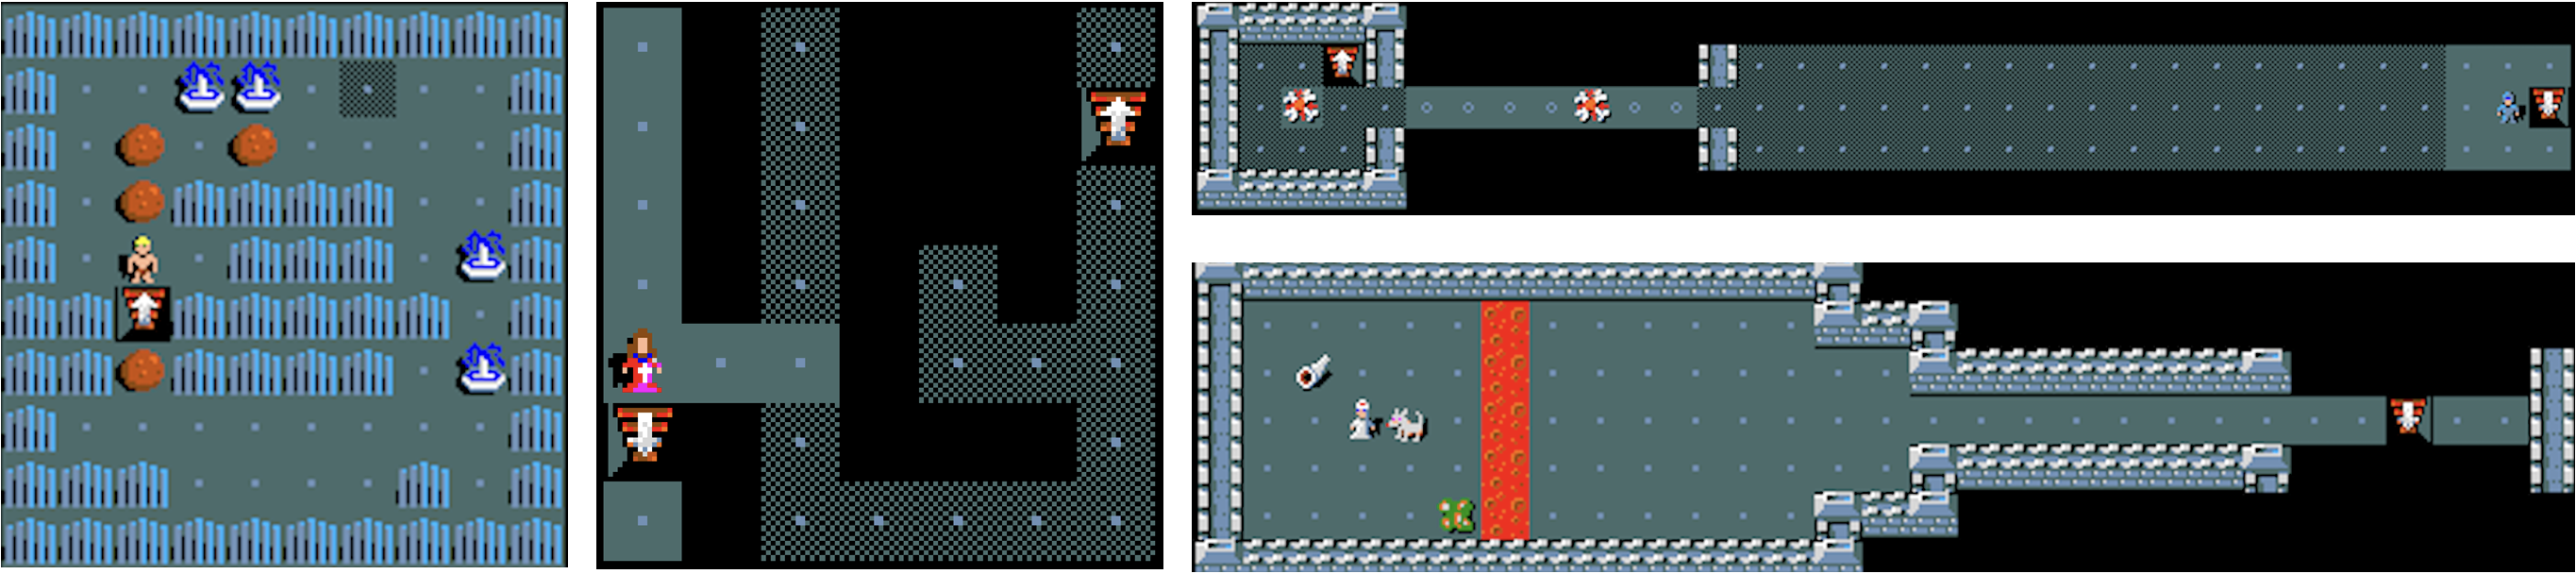
\includegraphics[width=\textwidth]{figs/emojis/maps.png}
    \caption{Overview of representative tasks used in MiniHack agent optimization process with AutoLibra. 
    From left to right, up to down: (1) \emph{Boxoban}, (2) \emph{MazeWalk}, (3) \emph{Corridor Fight}, and (4) \emph{Quest}.}
    \label{fig:minihack_maps}
\end{figure}

This section discusses the rules and implementation details of MiniHack, another task environment used in experiments in Section 4. Similarly to Baba is AI, MiniHack is derived from a grid-based puzzle video game (NetHack), and was originally implemented as part of the BALROG \cite{paglieri2024balrog} agent benchmark.

MiniHack is a grid navigation game expressed in text similar to baba-is-ai, consisting of a procedurally generated environment that requires the agent to navigate a space consisting of various agent roles, creatures, items, and tasks to reach a goal \cite{samvelyan2021minihackplanetsandboxopenended}. Given its plasticity and abundant elements, MiniHack is more complex, challenging, and diversified than baba-is-ai; this is reflected in a lower success rate for agents on MiniHack versus Baba is AI, with a baseline agent task completion rate of 10\% on MiniHack vs 33\% on baba-is-ai \cite{paglieri2024balrog}.

Similar to our experiments with baba-is-ai, the Ladder improvement process for MiniHack also follows the algorithm detailed in Appendix \ref{appendix:algo1}. Two full iterations of agent improvement with AutoLibra were performed on MiniHack. Four representative tasks for MiniHack are used in iterative metric improvement, with the remainder held out for evaluation. The agent is evaluated on the MiniHack environment and any changes to the agent code at the beginning of each iteration, and the environment score, trajectory performance, and other metrics are recorded at the end of each iteration. GPT-4o-241120 is used as the agent model.\\

The four selected representative tasks each contain a unique subset of subtasks evaluating an agent's capability. Figure \ref{fig:minihack_maps} shows an example for each task, and from left to right, up to down, these maps respectively represent Boxoban, MazeWalk, Corridor Fight, and Quest. 

\textbf{Boxoban} is a box-pushing puzzle game inspired by Sokoban, rendered within the MiniHack environment. To succeed in Boxoban, the agent needs to push the four boulders (orange balls) onto the four fountains (blue icons), and partial credit will be awarded for pushing some of the boulders onto the fountains. Boxoban tests the agent's capability in strategic planning and rule-following.
\newline
\\
\textbf{MazeWalk} is a game that requires the agent to explore unknown dark spaces to find the target exit staircase (the icon with a downward arrow). Two challenges for MazeWalk are fog of war -- the agent initially lacks information about areas of the map it hasn't visited, and must explore to discover the map and maze layout, and darkness -- even if the agent has visited a block, the block will become 'dark' as the agent walks away and it passes out of view, retaining information about its layout but not any enemies or items present. Thus, MazeWalk tests the agent's capability in map memory and strategic searching.
\newline
\\
\textbf{Corridor Fight} is a game that requires the agent to explore an unknown dark corridor map to find the target exit staircase while engaging or avoiding giant rat enemies. Corridor Fight tests the agent's capability in memory, space awareness, hazard awareness, and strategic combat.
\newline
\\
\textbf{Quest} requires the agent to use a tool to help itself cross an otherwise impassable wall of lava, survive randomly generated monsters, and search for the target exit staircase. As the most subtask-rich and randomized game, it tests the agent's abilities to recognize and utilize tools, understand its role and special power, and strategically survive from monsters.

In all tasks, the agent is provided observations in a text form, which includes the current state of the game field, the currently active rules, and relative locations of obstacles to the active player character in terms of shortest Manhattan distance. This is done to make the environment compatible with purely text-based language models.

The environment is limited to 100 steps per task episode to avoid tasks being solved by random walks.